\documentclass[10pt, a4paper]{article}

%\usepackage[paper=a4paper, left=1.5cm, right=1.5cm, bottom=1.5cm, top=3.5cm]{geometry}
\usepackage[paper=a4paper]{geometry}
\usepackage[latin1]{inputenc}
\usepackage[T1]{fontenc}
\usepackage[spanish]{babel}
\usepackage{indentfirst}
\usepackage{fancyhdr}
\usepackage{latexsym}
\usepackage{lastpage}
\usepackage[colorlinks=true, linkcolor=blue]{hyperref}
\usepackage{calc}
\usepackage{paralist}
\usepackage{caratula}
%\usepackage[plain,noline,linesnumberedhidden, noend]{algorithm2e}
%\usepackage[plain,noline,linesnumbered, noend]{algorithm2e}
\usepackage[plain,noline,noend]{algorithm2e}
\usepackage{graphicx}
\usepackage{caption}
\usepackage{subcaption}
\usepackage{amsmath}
\usepackage{float}
\usepackage{ulem}

\newcommand{\f}[1]{\text{#1}}
\newcommand{\call}[1] {\textsc{#1}}
\newcommand{\tab}[1]{\Indp \Indp #1 \Indm  \Indm}
\newcommand{\tabSpace}[1]{\Indp \Indp \; #1 \Indm \Indm \;}
\newcommand{\si}[2]{ {\bf si} (#1)\; \tab {#2} }
\newcommand{\sino}[1]{ {\bf sino}\; \tab {#1} }
\newcommand{\sinosi}[2]{ {\bf sino, si #1}\; \tab {#2} }
\newcommand{\mientras}[2] {  {\bf mientras} (#1) \; \tabSpace  {#2} }
\newcommand{\funcion}[3] { 	\KwSty{\call{#1}(#2)}\; \tabSpace  {#3} \KwSty{\call{Fin Funcion}} \newline }
\newcommand{\funcionConResultado}[4] {      \KwSty{\call{#1}(#2) $\rightarrow$ #3}\; \tabSpace  {#4} \KwSty{\call{Fin Funcion}} \newline }
\newcommand{\porcada}[3] { {\bf por cada } #1 {\bf en} #2 \; \tabSpace {#3} }
\newcommand{\para}[4] { {\bf para } #1 {\bf desde} #2 {\bf hasta} #3\; \{ \; \tab{#4}\}\; }
\newcommand{\paracada}[3] { {\bf para cada } #1 {\bf $\in$} #2 \; \tabSpace {#3} }
\newcommand{\devolver}[1] { {\bf devolver} #1\;}



\sloppy


\hypersetup{%
 % Para que el PDF se abra a pagina completa.
 pdfstartview= {FitH \hypercalcbp{\paperheight-\topmargin-1in-\headheight}},
 pdfauthor={C\'atedra de Algoritmos y Estructuras de Datos III - DC - UBA},
 pdfkeywords={Trabajo Pr\'actico 3},
 pdfsubject={}
}

\parskip=5pt % 10pt es el tama\~no de fuente

% Pongo en 0 la distancia extra entre itemes.
\let\olditemize\itemize
\def\itemize{\olditemize\itemsep=0pt}

% Acomodo fancyhdr.
\pagestyle{fancy}
\thispagestyle{fancy}
\addtolength{\headheight}{1pt}
\lhead{Base de Datos}
\rhead{TP2}
\cfoot{\thepage /\pageref{LastPage}}
\renewcommand{\footrulewidth}{0.4pt}

\author{Base de Datos, DC, UBA.}
\date{}
\title{}

\begin{document}

%Pagina de titulo e indice
\thispagestyle{empty}
\materia{Base de datos}
\submateria{TP2}
\titulo{}
\grupo{NN\_3}
\integrante{Sergio Gonz\'alez}{723/10}{sergiogonza90@gmail.com}
\integrante{Gino Scarpino}{392/08}{gino.scarpino@gmail.com}
\maketitle

\tableofcontents

\SetAlgoSkip{bigskip}
\NoCaptionOfAlgo
\DontPrintSemicolon
\SetAlFnt{\ttfamily}

\newpage

\section{Introducci\'on}

	\quad Es fundamental para cualquier motor de bases de datos, poseer un planificador para resolver consultas lo m\'as eficiente posible. Medir el costo de un m\'etodo de evaluaci\'on puede ser muy complejo, pero como se indica en el paper de Piatetsky-Shapiro, aproximadamente son las cantidad de operaciones de entrada y salida en disco que el motor realiza. Por eso mismo, se trata de minimizar estas operaciones.


\quad Una de las formas de poder minimizar estas operaciones, es conocer aproximadamente cual puede ser la distribuci\'on de un set de datos, y de esta forma poder estimar cuantas tuplas se obtendr\'a por el hecho de aplicar un filtro (WHERE) u otro que lo cumplan. El hecho de poder minimizar las tuplas resultantes que se obtendr\'an en una consulta, puede hacer que al momento de materializar la misma (por ejemplo en caso de tener que hacer un JOIN posterior) haga que las bajadas a disco de las tuplas se minimizen considerablemente.


\quad Si bien computar la distribuci\'on exacta de un set de datos puede ser muy costoso, existen m\'etodos con el cual se puede aproximar dichas distribuciones y de esa forma poder decidir cual es el mejor camino a seguir al momento de tener que resolver una consulta.




\section{Estimadores }

*******************\\
Aca no se si habria que explicar cada estimador.. tecnicamente no lo pide el enunciado.. asi q esto se podria obviar :P, si hay q explicar mas adelante el estimadir propio\\
*******************

\section{An\'alisis de m\'etodos}

	\subsection{Distribuciones conocidas}
	
		\subsubsection{Distribuciones normal (Ejemplos)}	
		
			La distribuci\'on normal es una de las distribuciones que mas aparece en la vida real. A continuaci\'on se presentan 2 ejemplos de la misma.
	
	\subsubsection*{Altura de una persona}
	
		Es ampliamente conocido que las caracter\'isticas morfol\'ogicas de individuos, tales como la estatura, siguen el modelo normal en todo el mundo. En general, se puede pensar la altura de las personas suele estar entre 1-70 y 1.75 metros, debido a que en la mayor\'ia de los casos es as\'i. Es minor\'ia las personas que midan menos de 1.50, y a la vez no hay tampoco demasiadas personas que superen los 2 metros. Haciendo un muestreo poblacional y realizando un histograma del mismo se puede visualizar esta intuici\'on.
		
\begin{figure}[H]
  \begin{center}
    %\includegraphics[scale=.41,angle=-90]{imgenes/normal_ejemplo1.png}
    \includegraphics[scale=.40]{imagenes/normal_ejemplo1.png}
    \caption{Histograma altura} 
    \label{fig:normal_ejemplo1}
  \end{center}
\end{figure}		
		
Se puede ver como para el muestreo realizado, la mayor\'a de las personas caen en la altura entre 1.70 y 1.80 metros, dando como resultado aproximadamente, una normal con media 1,75 y desv\'io standard 0.64.

\newpage

	\subsubsection*{IQ de una persona}
	
		Otro ejemplo muy conocido es el coeficiente intelectual de las personas, conocido como IQ. Seg\'un el siguiente ranking, vemos que una inteligencia normal deber\'ia estar entre los 90 y los 109 de coeficiente intelectual. Por lo que es de esperar que la mayor parte de la poblaci\'on este en este promedio.
\newline

\begin{tabular}{| l | l |}
\hline
IQ Range & Clasificaci\'on \\
\hline
130 o mas & Muy Superior \\
\hline
120\--129	& Superior \\
\hline
110\--119	& Arriba del promedio \\
\hline
90\--109	& Promedio \\
\hline
80\--89	& Abajo del Promedio \\
\hline
70\--79	& L\'imite \\
\hline
69 o menos & Extremadamente bajo \\
\hline
\end{tabular}
\newline

\noindent 
Veamos un histograma sobre el muestreo del IQ de los individuos de una poblaci\'on. 


\begin{figure}[H]
  \begin{center}
    %\includegraphics[scale=.41,angle=-90]{imgenes/normal_ejemplo1.png}
    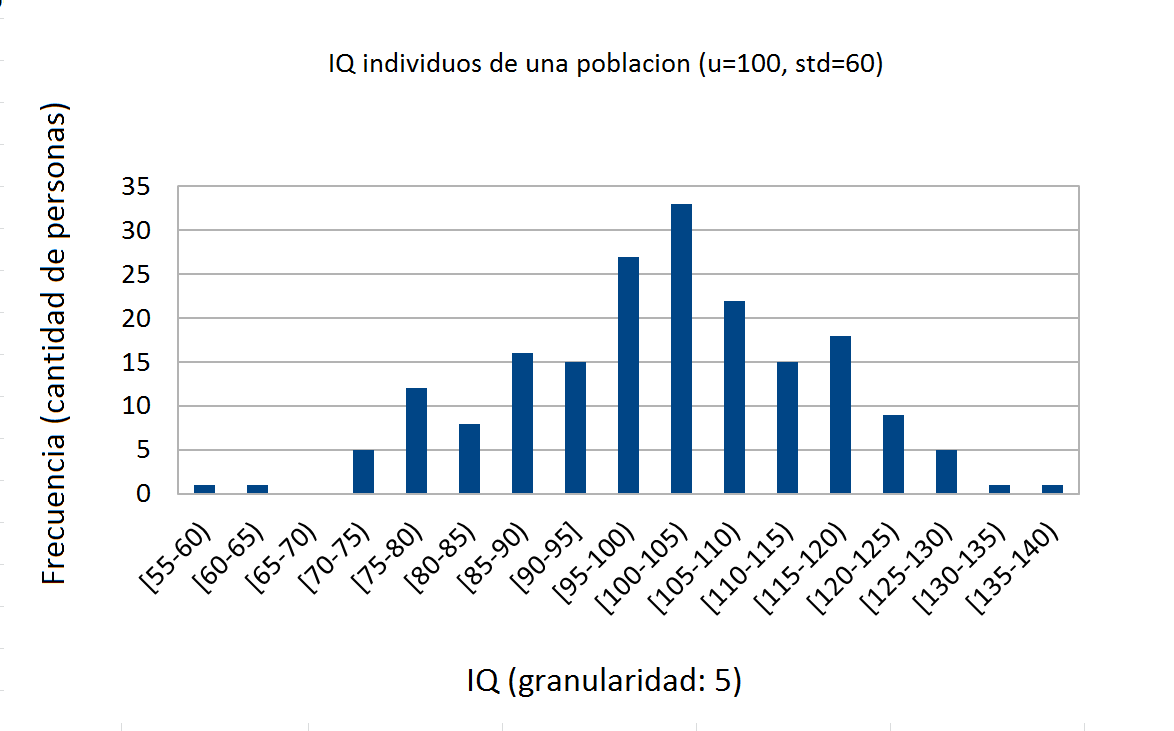
\includegraphics[scale=.40]{imagenes/normal_ejemplo2.png}
    \caption{Histograma IQ} 
    \label{fig:normal_ejemplo2}
  \end{center}
\end{figure}	

En la figura \ref{fig:normal_ejemplo2}, podemos un ver como, efectivamente, la mayor\'ia de la poblaci\'on se centra en un IQ de 100, con una desv\'io al rededor de 20.		
		

\end{document}